\begin{minipage}{.46\textwidth}
  \tdplotsetmaincoords{100}{0}
  \begin{tikzpicture}[scale=0.55, tdplot_main_coords]
    \pgfmathsetmacro{\R}{4}
    \pgfmathsetmacro{\Rs}{2}
    \pgfmathsetmacro{\HW}{4}
    \pgfmathsetmacro{\HWs}{0.2}
    \pgfmathsetmacro{\HC}{6}
    % water
    \fill[cyan!30] plot[variable=\x,domain=0:180,smooth] ({\R*cos(\x)},{\R*sin(\x)},0)
    --
    plot[variable=\x,domain=180:360,smooth] ({\R*cos(\x)},{\R*sin(\x)},\HW)
    -- cycle;
    \draw[black] plot[variable=\x,domain=0:360,smooth,samples=51]
    ({\R*cos(\x)},{\R*sin(\x)},\HW);
    \fill[black!20] plot[variable=\x,domain=0:180,smooth] ({\Rs*cos(\x)},{\Rs*sin(\x)},0)
    --
    plot[variable=\x,domain=180:360,smooth] ({\Rs*cos(\x)},{\Rs*sin(\x)},\HWs)
    -- cycle;
    \draw[black] plot[variable=\x,domain=0:360,smooth,samples=51]
    ({\Rs*cos(\x)},{\Rs*sin(\x)},\HWs);
    \draw[black] plot[variable=\x,domain=0:180,smooth]
    ({\Rs*cos(\x)},{\Rs*sin(\x)},0);
    \draw (\Rs,0,0) -- (\Rs,0,\HWs);
    \draw (-\Rs,0,0) -- (-\Rs,0,\HWs);
    \draw [ thick , densely dashed ] (0,0,\HW) -- (0+1.38*0.886,0,\HW-1.38*0.5);
    \node[anchor=north,font=\footnotesize] at (1.4,0,\HW+0.5) {$\mathrm{R_y}$};
    \draw (0,0,\HW-0.2) -- (0,0,\HW+0.2);
    \draw (0-0.2,0,\HW) -- (0+0.2,0,\HW);
    % "invisible" lined
    \draw[black]
    plot[variable=\x,domain=180:360,smooth]
    ({\R*cos(\x)},{\R*sin(\x)},0);
    % visible cylinder lines
    \draw plot[variable=\x,domain=0:180,smooth]
    ({\R*cos(\x)},{\R*sin(\x)},0)
    --
    plot[variable=\x,domain=180:360,smooth]
    ({\R*cos(\x)},{\R*sin(\x)},\HC) -- cycle;
    \draw plot[variable=\x,domain=0:180,smooth]
    ({\R*cos(\x)},{\R*sin(\x)},\HC);
    \node[anchor=north,font=\footnotesize] at (0,0,0.65) {Electrode};
    \node[anchor=north,font=\footnotesize] at (0,0,2.5) {Solution of A and B};
    \coordinate (O) at (-6,1,0);
    \draw[thick,->] (-6,1,0) -- (-6,1,0+1);
    \draw[thick,->] (-6,1,0) -- (-6+0.866,1,0-0.5);
    \draw[thick,->] (-6,1,0) -- (-6-0.886,1,0-0.5);
    \node[anchor=north,font=\footnotesize] at (-6-1.3,1,0-0.2) {$x$};
    \node[anchor=north,font=\footnotesize] at (-6+1.2,1,0-0.2) {$y$};
    \node[anchor=north,font=\footnotesize] at (-6,1,0+1.7) {$z$};
  \end{tikzpicture}%
\end{minipage}
\begin{minipage}{.13\textwidth}
  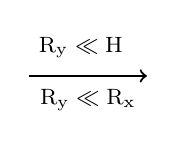
\begin{tikzpicture}
    \draw[thick,->] (0,0) -- (1.5,0);
    \node[anchor=north,font=\footnotesize] at (0.66,0.62) {$\mathrm{R_y}\ll \mathrm{H}$};
    \node[anchor=north,font=\footnotesize] at (0.75,-0.05) {$\mathrm{R_y}\ll \mathrm{R_x}$};
  \end{tikzpicture}%
\end{minipage}
\begin{minipage}{.39\textwidth}
  \begin{tikzpicture}
    \fill[cyan!30]
    decorate[ragged border]{
        (0,2.2) -- (5,2.2)
      }
    (0,2.2) -- (5,2.2)--(5,0)--(3.5,0)-- (3.5,0.6) -- (1.5,0.6)-- (1.5,0) -- (0,0) -- (0,2.2);
    \fill[black!20]
    (1.5,0.6) -- (3.5,0.6)--(3.5,0)--(1.5,0);
    \draw (1.5,0) -- (1.5,0.6) -- (3.5,0.6) -- (3.5, 0);
    \draw (0,2.5) -- (0,0) -- (5,0) -- (5,2.5) -- (0,2.5);
    \draw[>=triangle 45, <->] (0,2.8) -- (5,2.8);
    \draw[>=triangle 45, <->] (-0.3,0.6) -- (-0.3,2.2);
    \node[anchor=north,font=\footnotesize] at (2.5,3.4) {$\mathrm{2\mathrm{R_x}}$};
    \node[anchor=north,font=\footnotesize] at (-0.6,1.6) {$\mathrm{H}$};
    \node[anchor=north,font=\footnotesize] at (-0.6,0.6) {$\mathrm{L}$};
    \draw[>=triangle 45, <->] (-0.3,0) -- (-0.3,0.6);
    \draw [ thick , densely dashed ] (1.5,0.6) -- (0,0.6);
    %\draw[-stealth] (6.5,0.75) -- (7.2,0.75);
    %node[anchor=west,font=\footnotesize]{\SI{5}{\liter/\minute}};
    %\draw (5,0) -- (5,-0.5) -- (7,-0.5) -- (7,0.5);
    %\draw (7, 1.5) -- (7,2) -- (6,2);
    %\draw[color=black] (7,1) circle [radius=0.5];
    \node[anchor=north,font=\footnotesize] at (2.5,0.55) {Electrode};
    \node[anchor=north,font=\footnotesize] at (2.5,1.65) {Solution of A and B};
    %\node[anchor=north,font=\normalsize] at (7,1.25){\textbf{$\mathrm{V}$}};
    %\draw [line width=0.3mm] (-0.8,0.6) -- (-0.8,2.2);
    %\foreach \x in {0,...,5}
    %    \draw [line width=0.3mm] (-0.9,0.6+\x*0.32) -- (-0.7,0.6+\x*0.32);
    %\node[anchor=north,font=\footnotesize] at (-1.55,0.85) {$x=0$};
    %\node[anchor=north,font=\footnotesize] at (-1.55,2.45) {$x=\mathrm{\mathrm{R_x}}$};
  \end{tikzpicture}%
\end{minipage}
